\documentclass{uni_tue_template}

\usetikzlibrary{patterns}
% content of left head area e.g. subject like ETI
\def \headLeft{MatheIII Skript}

% content of center head area, used for names
\def \names{David Morgenstern \& Yannick Runge}

% content of right head area e.g. semester like WiSe 2012/13
\def \headRight{2013/2014}

\newboolean{compileall}
\setboolean{compileall}{false}

\usepackage{hyperref}
\usepackage{multirow}
\usepackage{color}

\title{Mathematik III Prof. Hauck}
\author{David Morgenstern \& Yannick Runge}

\begin{document}
\ifthenelse{\boolean{compileall}}{
	\thispagestyle{empty}
	\maketitle
	\tableofcontents
	\thispagestyle{empty}
	\cleardoublepage
	\setcounter{page}{1}
	\foreach \inputpage in {1,...,9} {
		\input{Math_C\inputpage}
	}
}{
	\newpage
\section{Mehrdimensionale Analysis}
	Folgen: $ (a_i)_{i\in\mn} $, $ a_i\in\mr $\\
	Funktionen: $ f=\mr^n\rightarrow\mr^m $\\
	Hier $ \mr^n $ Zeilenvektoren\\
	Lönge: $ ||x||=\sqrt{(x|x)}=\sqrt{\limsum{i=1}{n}x_i^2} $\\
	$ x=\lrv{x_1\\\vdots\\x_n} $\\
	Abstand $ ||x-y||=\sqrt{\limsum{i=1}{n}(x_i-y_i)^2} $
	
\subsection{Defninition}
	$ (a_i)_{i\in\mz} $ Folge in $ \mr^n $ konvergiert gegen $ c\in\mr^n $\\
	$ \Leftrightarrow\ \forall\epsilon>0\ \exists N(\epsilon)\in\mn\ \forall i\geq N(\epsilon) $\\
	$ ||a_i-c||<\epsilon $\\
	$ ((a_i)\rightarrow c) $\\
	Ist $ a_i=\lrv{a_i^{(1)}\\\vdots\\a_i^{(n)}},\ c=\lrv{v^{(1)}\\\vdots\\c^{(n)}} $, so gilt:\\
	$ (a_i)\rightarrow c\ \Leftrightarrow\ \lrr{a_i^{(j)}}\ouset{\longrightarrow}{}{i\rightarrow\infty}c^{(j)} $ für $ j=1,...,n $\\
	Bsp.: $ a_i=\lrv{1/i\\0\\1-2/i} $, $ i\in\mn $\\
	$ (a_i)\ouset{\longrightarrow}{}{i\rightarrow\infty}\lrv{0\\0\\1} $
	
\subsection{Beispiel für Funktionen}
	\subExBegin{a)}
		\item  lineare Abbildung $ \mr^n\rightarrow\mr^n $ sind Funktionen $ f\lrv{x_1\\\vdots\\x_n}^t=\lrr{A\cdot\lrv{x_1\\\vdots\\x_n}}^t=\lrv{a_{11}x_1+...+a_{1n}x_n\\a_{m1}x_1+...+a_{mn}x_n}^t$\\
		affine Abbildung $ \lrv{...+b_1\\...+b_n} $
		\item  $ f:D\mpo\mr^n\rightarrow\mr $ \textbf{skalare Funktion}\\
		z.B. $ f(x_1,x_2,x_3)=x_1^3+x_2^2+x_3^2 $, $ D=\mr^3 $\\
		$ f(x,y)=\frac{2xy}{x^2+y^2} $, $ D=\mr^2\mnot\lrc{(0,0)} $\\
		Graphische Darstellung für mögliche Funktionen $ f:D\mpo\mr^2\rightarrow\mr $
		
		\begin{tikzpicture}
			\draw [->] (0,0) -- (3,0) node [anchor=south west] {$ y $};
			\draw [->] (0,0) -- (0,3) node [anchor=south east] {$ z $};
			\draw [->] (0,0) -- (-1.5,-1.5) node [anchor=north east] {$ x $};
			\draw [dotted] (0,0) -- (0.5,-0.5) -- (0.5,1.5) -- (0,2) node [anchor=east] {$ f(x,y) $};
			\fill (0.5,-0.5) circle [radius=1.5pt];
			\fill (0.5,1.5) circle [radius=1.5pt];
		\end{tikzpicture}
		
		\item  $ f:D\mpo\mr^n\rightarrow\mr^m $, $ m>1 $ \textbf{vektorwertige} Funktionen.\\
		$ f(x_i,...,x_n)=(f(x_1,...,x_n),...,f_m(x_1,...,x_n)) $ mit $ f_1,...,f_m $ skalare Funktionen
		
		\item $ f:D\mpo\mr\rightarrow\mr^2 $ \textbf{ebene Kurven},\\
		z.B. $ f:\begin{cases}[0,2\pi[\rightarrow\mr^2\\t\mapsto(\cos(t),\sin(t))\end{cases} $
		
		% TODO insert circle graphic
		
		Lissajon- Kurven z.B. $ f:\begin{cases}t\rightarrow(\sin(2t),\sin(3t))\\\mr\rightarrow\mr^2\end{cases} $
		
		$ f:D\mpo\mr\rightarrow\mr^3 $ \textbf{Raumkurve}
	\subExEnd

\subsection{Definition: Adhärenzpunkt}
	\subExBegin{a)}
		\item $ a\in\mr^n $ heißt \textbf{Adhärenzpunkt}, falls Folge $ (d_i)_{i\in\mn} $ existiert mit $ d_i\in D $ und $ (d_i)\rightarrow a $.\\
		Klar: Jeder Punkt in $ D $ ist Adhärenzpunkt von $ D $.
		
		\item $ f:D\mpo\mr^n\rightarrow\mr^m $, $ a $ Adhärenzpunkt von $ D $, wenn $ \limlim{x\rightarrow a}f(x)=c'(\in\mr^m) $, falls für jede Folge $ (d_i) $, $ d_i\in D $ mit $ \limlim{i\rightarrow\infty}d:i=a $ gilt $ \limlim{i\rightarrow\infty}f(d_i)=c $.\\
		Äquivalent: $ \forall\epsilon >0\ \exists\delta>0\ \forall x:||x-a||<\delta\Rightarrow||f(x)-c||<\epsilon $
		
		\item $ a\in D:\ f:D\mpo\mr^n\rightarrow\mr^m $ ist \textbf{stetig} in $ a $ $ \Leftrightarrow $ $ \lim\limits_{x\rightarrow a}f(x)=f(a) $.
	\subExEnd

\subsection{Bemerkung}
	$ f:D\mpo\mr^n\rightarrow\mr^m $. $ f(x)=\lrv{f_y(x)\\...\\f_m(x)}\in\mr^m$\\
	Dann: $ f_i:D\mpo\mr^n\rightarrow\mr $\\
	$ \lim\limits_{x\rightarrow\infty}f(x)=\lrv{c_1\\\vdots\\c_m}\Leftrightarrow\lim\limits_{x\rightarrow a}f_i(x)=c $ für $ i=1,...,m $.\\
	Insbesondere: $ f $ ist stetig in $ a\in D $ $ \Leftrightarrow $ $ f $ ist stetig in $ a\in D $, $ i=1,...,m $.\\
	Daher: Skalare Funktion $ f:D\mpo\mr^n\rightarrow\mr $ besonders wichtig.
	
\subsection{Bemerkung}
	Monom: $ f(x_1,...,x_n)r\cdot x_1^{m_1}...x_n^{m_n} $ $ (r\in\mr) $\\
	$ f:\mr^n\rightarrow\mr $\\
	Endliche Summen von Monomen = \textbf{Polynome} (Polynomfunktionen)\\
	z.B. $ f(x_1,x_2,x_3)=x_1^5+x_2x_3-\pi x_2x_3^4 $\\
	Polynome sind stetig\\
	Summen, Produkte, Quotienten, Hintereinanderausführungen von stetigen (skalaren) Funktionen sind stetig.
	
\subsection{Definition}
	\begin{enumerate}[a)]
		\item $ a\in\mr^n $, $ r\in\mr $, $ r>0 $\\
		$ K(a,r)=\lrc{x\in\mr^n:||x-A||<R} $\\
		\textbf{offene Kugel} um $ a $ mit Radius $ r $.
		
		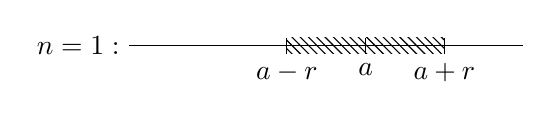
\begin{tikzpicture}
			\draw (0,0) node [anchor=east] {$ n=1: $} -- (5,0);
			\draw(2,.1) -- (2,-.1) node [anchor=north] {$ a-r $};
			\draw(4,.1) -- (4,-.1) node [anchor=north] {$ a+r $};
			\draw(3,.1) -- (3,.-.1) node [anchor=north] {$ a $};
			\pattern [pattern=north west lines] {(2,-.1) -- (4,-.1) -- (4,.1) -- (2,.1)};
		\end{tikzpicture}
		
		offenes Intervall $ ]a-r,a+r[ $
		%Graphics 02
		Adhärenzpunkte von $ K(a,r)=\lrc{x\in\mr^n:||x-a||\leq r} $ \textbf{abgeschlossene Kugel}.
		
		\item  $ D\mpo\mr^n $ heißt \textbf{offen}, falls es zu jedem $ a\in D $ ein $ r(a)>0 $ gibt, so dass $ K(a,r(a))\mpo D $\\
		Offene Kugel ist offen
		% Graphics 03
	\end{enumerate}

\subsection{Definition: Jacobi- Matrix}
	$ f:D\mpo\mr^n\rightarrow\mr $,$ D $ offen, $ a=(a_1,...,a_n)\in D $
	\begin{enumerate}[a)]
		\item $ f $ heißt \textbf{partiell differenzierbar nach }$ \mathbf{x} $, an der Stelle $ a $, falls gilt
		\[ \lim\limits_{x_j\rightarrow a_j}\dfrac{f(a_1,...,a_{j-1},x_j,a_{j+1},...,a_n)-f(a_1,...,a_n)}{x_j-a_j} \]
		existiert.\\
		\textbf{Partielle Ableitung} von $ f $ nach $ x_j $ an der Stelle $ a $, $ \frac{\partial f(a)}{\partial x_j} $ ($ n=1:\ \lim\limits_{x\rightarrow a}\frac{f(x-f(a))}{x-a}\\
		\frac{\partial f}{\partial x}(a)\leftrightarrow f'(a)$)
		
		\item  Ist $ f $ partiell nach allen $ x_j $ and er Stelle $ a $ differenzierbar, so heißt ($ \frac{\partial f}{\partial x_n}(a),...,\frac{\partial f}{\partial x_n}(a)=\mbox{Grad }f(a) $), der \textbf{Gradient} von $ f $ an der Stelle $ a $.\\
		($ n=1:(\mbox{Grad }f(a)=(f'(a)) $)
		
		\item  Ist $ f $ an allen $ a\in D $ partiell nach allen $ x_j $ differenzierbar, so sind $ \frac{\partial f}{\partial x_j}:\begin{cases}D\mpo\mr^n\rightarrow\mr\\ a\mapsto\frac{\partial f}{\partial x_j}(a)\end{cases} $ selbst Funktionen, die \textbf{partiellen Ableitungen} von $ f $, zusammengefasst im Grad $ f=\lrr{\frac{\partial f}{\partial x_i},...,\frac{\partial f}{\partial x_n}} $ \textbf{Gradient} von $ f $.\\
		ist $ f:D\mpo\mr^n\rightarrow\mr^m $ $ f(x)=\lrv{f_1(x)\\\vdots\\f_m(x)}\quad f_i:D\rightarrow\mr $\\
		Sind alle $ f_i $ partiell differenzierbar nach allen Variablen, so ist
		\[
		\begin{pmatrix}
		\dfrac{\partial f_1}{\partial x_1}&...&\dfrac{\partial f_1}{x_n}\\
		\dfrac{\partial f_2}{\partial x_1}&...&\dfrac{\partial f_2}{\partial x_n}\\
		&\vdots&\\
		\dfrac{\partial f_m}{\partial x_1}&...&\dfrac{\partial f_m}{\partial x_n}
		\end{pmatrix}
		\]
		\textbf{Jacobi- Matrix} von $ f $.
	\end{enumerate}

\subsection{Beispiel}
	$ f:\mr^2\rightarrow\mr $ $ f(x_1,x_2)=\sin(x_1\cdot x_2) $\\
	Partielle Ableitungen an der Stelle $ \underbrace{(\pi, 1}_{a} $\\
	$ \frac{\partial f}{\delta x_1}(\pi, 1)=\lim\limits_{x_1\rightarrow\pi}\frac{f(x_1,1)-f(\pi, 1)}{x_1-\pi}=\lim\limits_{x_1\rightarrow\pi}\frac{\sin(x_1)-\sin(\pi)}{x_1-\pi}=\sin'(\pi)=\cos(\pi)=-1 $\\
	$ \frac{\partial f}{\partial x_2}(\pi, 1)=(\sin'(\pi x_2))(1)=(\pi\cdot\cos(\pi\cdot x_2))(1)=\pi\cdot\cos(\pi)=-\pi $
	
	Allgemein: Partielle Ableitung an einer beliebigen Stelle $ (x_1,x_2) $:\\
	$ \frac{\partial f}{\partial x_1}=x_2\cdot\cos(x_1\cdot x_2) $\\
	$ \frac{\partial f}{\partial x_2}=x_1\cdot\cos(x_1\cdot x_2) $\\
	$ \grad(f)=(x_2\cdot\cos(x_1\cdot x_2), x_1\cdot\cos(x_1\cdot x_2)) $
	
	Im 1- dimensionalen: $ f $ differenzierbar $ \Rightarrow $ $ f $ stetig.
	
	Es gibt Bsp. von $ f\mr^2\rightarrow\mr $, so dass an der Stelle $ a\in\mr^2 $ alle partiellen Ableitungen existieren, aber $ f $ nicht stetig in $ a $, z.B.:
	\[f(x_1,x_2)=\begin{cases}\dfrac{x_1x_2}{x_1^2+x_2^2}\mbox{ falls } (x_1,x_2)\neq(0,0)\\
	0\mbox{ falls }(x_1,x_2)=(0,0) \end{cases}\]
	
	\textbf{Bsp.:} $ f((x,y))=1-\min(|x|,|y|) $ Partielle Ableitung in $ (0,0) $ existieren, aber es gibt keine Tangentialebene an $(0,0)$.\\
	Gutartig: $ f((x,y))=1-x^2-y^2 $
	
	\textbf{Also:} Partielle Diffbarkeit ist zu schwach, um Stetigkeit oder Existenz von Tangentialebenen ($ n=2 $) folgern zu können.
	
\subsection{Definition}
	\begin{enumerate}
		\item $ f: D\mpo\mr^n\rightarrow\mr $, $ D $ offen, heißt \textbf{stetig differenzierbar}, wenn $ f $ in $ D $ überall partiell differenzierbar ist \textbf{und} $ \frac{\partial f}{\partial x_j}:D\rightarrow\mr $ sind stetig für $ j=1,...,n $.
		
		\item  $ f $ heißt \textbf{2- mal stetig differenzierbar}, falls $ f $ stetig differenzierbar ist und alle partiellen Ableitungen stetig differenzierbar sind.\\
		Partielle Ableitung von $ \frac{\partial f}{\partial x_j} $ und $ x_k:\frac{\partial^2 f}{\partial x_k\partial x_j} $\\
		$ k=j $ $ \frac{\partial^2 f}{(\partial x_j)^2} $
		
		\item Analog: $ s $- mal stetig differenzierbar, $ \frac{\partial^s f}{\partial x_{j_{s}}\partial x_{j_{s-1}}...\partial x_{j_{1}}} $
	\end{enumerate}
	
\subsection{Beispiele}
	\subExBegin{a)}
		\item Polynomfunktionen sind $s$-mal stetig diffbar für alle $s\in\mn$ (Partielle Ableitungen sind wieder Polynomfunktionen)
			
			z.B: $f(x_1,x_2,x_3)=x_1^{15}x_2^7+3x_1x_2x_3$\\
			$\frac{\partial f}{\partial x_1} = 15x_1^{14}x_2^7+3x_2x_3$\\
			$\frac{\partial f}{\partial x_3} = 3x_1x_2$
		\item Ebenso Funktionen wie $f\lrr{x_1,x_2} = \sin\lrr{x_1\cdot x_2}+e^{x_2}$\\
			$\frac{\partial f}{\partial x_1} = x_2\cdot\cos\lrr{x_1x_2}$\\
			$\frac{\partial f}{\partial x_2} = x_1\cdot\cos\lrr{x_1x_2}+e^{x_2}$\\
			$\frac{\partial^2f}{\lrr{\partial x_1}^2} = -x_2^2\cdot\sin\lrr{x_1,x_2}$\\
			$\frac{\partial^2f}{\lrr{\partial x_2}^2} = -x_1^2/sin\lrr{x_1,x_2}+e^{x_2}$\\
			$\frac{\partial^2f}{\partial x_2\partial x_1} = \cos\lrr{x_1x_2}-x_2x_1\sin\lrr{x_1x_2}$\\
			$\frac{\partial^2f}{\partial x_1\partial x_2} = \cos\lrr{x_1x_2}-x_1x_2\sin\lrr{x_1x_2}$
	\subExEnd

\subsection{Satz von Schwarz}
	$f:D\mpo\mr^n\rightarrow\mr$, $D$ offen, $2$-mal stetig diffbar\\
	$\Rightarrow \frac{\partial^2 f}{\partial x_i\partial x_j}=\frac{\partial^2 f}{\partial x_j\partial x_i}$ für alle $i,j$

\subsection{Satz}
	$D\mpo\mr^n$ offen, $f:D\rightarrow\mr$ stetig diffbar.\\
	Dann gilt für alle $a\in D$:\\
	$\limlim{x\rightarrow a} \frac{f\lrr{x}-f\lrr{a}-\lrr{\grad f}\lrr{a}\cdot\lrr{x-a}^t}{\lrabs{\lrabs{x-a}}}=0 (*)$\\
	Das heißt $f(x)$ wird in der Nähe von $a$ gut approximiert durch die affine Abbildung\\
	$l\lrr{x}=f\lrr{a}+\lrr{\grad f}\lrr{a}\cdot\lrr{x-a}^t=f\lrr{a}+\frac{\partial f}{\partial x_1}\lrr{a}\cdot\lrr{x_1-a_1}+\dots+\frac{\partial f}{\partial x_n}\lrr{a}\lrr{x_n-a_n}$\\
	$x=\lrr{x_1,\dots,x_n}, a=\lrr{a_1,\dots,a_n}$

	$n=1$: Entspricht (*) der Definition von Diffbarkeit\\
	$f:D\mpo\mr\rightarrow\mr$\\
	$\limlim{x\rightarrow a}\frac{f(x)-f(a)}{x_a} = f'(a)\Leftrightarrow\limlim{x\rightarrow a}\frac{f(x)-f(a)-f'(a)(x-a)}{x-a}=0 \Leftrightarrow\limlim{x\rightarrow a}\frac{f(x)-f(a)-f'(a)(x-a)}{\lrabs{x-a}}=0$\\
	$l(x)=f(a)+f'(a)(x-a)$ Tangente an $(a,f(a))$

	$n=2$:\\
	$E(x_1,x_2)=f(a)+\frac{\partial f}{\partial x_1}(a)(x_1-a_1)+\frac{\partial f}{\partial x_2}(a)(x_2-a_2)$\\
	Gleichung der Tangentialebene an $(a,f(a))$

\subsection{Beispiel}
	$f(x_1,x_2)=1-x_1^2-x_2^2$\\
	$\frac{\partial f}{\partial x_1} = -2x_1\quad\frac{\partial f}{\partial x_2}=-2x_2$\\
	$a=\lrr{\frac{1}{2},\frac{1}{2}}\;\; f(a)=\frac{1}{2}$\\
	$E\lrr{x_1,x_2}=\frac{1}{2} - \lrr{x_1-\frac{1}{2}}-\lrr{x_2-\frac{1}{2}}=\frac{3}{2}-x_1-x_2$

\subsection{Korollar}
	Ist $f$ stetig differenzierbar, so ist $f$ stetig.

\subsection{Definition: Hesse- Matrix}
	$ f: D\mpo\mr\rightarrow\mr $, $ D $ offen, $ f $ 2- mal stetig differenzierbar.\\
	Dann heißt die Matrix der zweiten partiellen Ableitung
	\[ H(f)=\lrr{\dfrac{\partial^2 f}{\partial x_i\ \partial x_j}}_{i,j=1,...,n} \]
	\textbf{Hesse- Matrix} von $ f $.\\
	Setzt man Punkt $ a\in D $ ein: $ H(f)(a) $ $ n\times n $- Matrix über $ \mr $.\\
	Nach 10.10: $ H(f)=H(f)^t $, $ H(f)(a)=H(f)(a)^t $\\
	$ H(f)(a) $ symmetrische Matrix.\\
	9.11: $ H(f)(a) $ hat $ n $ reelle Eigenwerte (inklusive Vielfachheit), diagonalisierbar,, charakteristisches Polynom zerfällt vollständig in Linearfaktoren.
	
\subsection{Definition: lokale Extremstellen}
	$ D\mpo\mr $ offen, $ f:D\rightarrow\mr $. $ a\in D $ heißt \textbf{lokale Maximum-/Minimumstelle}, wenn es eine Kugel $ K(a,r\mpo D) $ gibt mit $ f(x)\leq f(a) $ / $ f(x)\geq f(a) $ für alle $ x\in K(a,r) $. $ f(a) $ heißt dann lokales Maximum/Minimum von $ f $.\\
	(lokale \textbf{Extreme}, lokale \textbf{Extremstellen}).
	
\subsection{Satz}
	$ D\mpo\mr^n $, $ D $ offen, $ f:D\rightarrow\mr $.
	\begin{enumerate}[a)]
		\item Sei $ f $ stetig differenzierbar. Ist $ a $ lokale Extremstelle, so ist $ \grad f(a)=(0,...,0) $.
		\item  Sei $ f $ 2- mal stetig differenzierbar, $ \grad f(a)=(0,...,0) $.
		\begin{itemize}
			\item  Hat $ H(f)(a) $ lauter positive Eigenwerte, so ist $ a $ lokale Minimumsstelle.
			\item  Hat $ H(f)(a) $ lauter negative Eigenwerte, so ist $ a $ lokale Maximumsstelle.
			\item  Hat $ H(f)(a) $ sowohl positive als auch negative Eigenwerte, so ist $ a $ keine Extremalstelle
			\item Hat $ H(f)(a) $ nur nicht- negative (nicht- positive) Eigenwerte und falls 0 Eigenwerte ist, dann ist keine Aussage (aufgrund der Hesse- Matrix) möglich.\\
			(Vergleiche 1-dim Fall:\\
			$ H(f)(a)=f''(a)\ >0,<0,=0 $)
		\end{itemize}
	\end{enumerate}
	
	\textbf{Beweis:}
	\begin{enumerate}[a)]
		\item Folgt aus 1- dim. Fall (in jeder Koordinatenrichtung liegt Max oder Min vor.)
		\item  Folgt aus den mehrdimensionalen Satz von Taylor (1- dim. Satz von Taylor folgt)
	\end{enumerate}
	
\subsection{Beispiel}
	\begin{enumerate}[a)]
		\item $ f(x_1,x_2)=x_1^2+x_2^2 $\\
		$ \grad f=(2x_1,2x_1)=(0,0)\ \Leftrightarrow\ x_1=x_2=0 $\\
		$ H(f)=\lrv{2&0\\0&2}=H(f)(0,0) $ Eigenwerte alle positiv $ \Rightarrow $ lokales Minimum
		\item  $ f(x_1,x_2)=x_1^2-x_2^2 $\\
		$ \grad f=(2x_1-2x_2) =(0,0)$ $ \Leftrightarrow $ $ x_1=x_2=0 $\\
		$ H(f)=\lrv{2&0\\0&-2}=H(f)(0,0) $\\
		$ \Rightarrow (0,0) $ ist keine lokale Extremstelle.
		\item  $ f(x_1,x_2)=x_1^2+x_2^4+2x1 $\\
		$ \grad f=(2x_1+2,4x_2^3)=(0,0) $ $ \Leftrightarrow $ $ x_1=-1,\ x_2=0 $\\
		$ H(f)=\lrv{2&0\\0&12 x_2^2} $\\
		$ H(f)=(-1,0)=\lrv{2&0\\0&0} $\\
		Keine Aussage möglich.\\
		(Tatsächliches lokales Minimum)
	\end{enumerate}

\subsection{Geometrische Bedeutung des Gradienten}
	$ f:D\mpo\mr^n\rightarrow\mr $, $ D $ offen, $ a\in D $, $ \grad f(a)$ ist der Vektor, der in die Richtung des steilsten Anstiegs von $ f $ an der Stelle $ a $ zeigt.
	
	Bsp.: $ f(x,y)=1-x^2-y^2 $, $ a=(0,55,\ -0,65) $\\
	$ \grad(f)=(-2x,-3y) $, $ \grad(f)(a)=(-1,1,\ 1,3) $\\
	$ (a,f(a))\ouset{\longrightarrow}{}{\mbox{\scriptsize steilst. Anst.}} (a+t(-1,1,\ 1,3)) $, $ f(a+t(-1,1,\ 1,3)) $ für kleine $ t $ \textbf{infitessimale}.
}
\end{document}
